\chapter{A Graphical User Interface for SOSAA} \label{txt:sosaa-gui-chapter}

The SOSAA model has been under active use and development at the University of Helsinki since its initial publication in 2011 \cite{sosa-description-2011}. It consists of several coupled modules that model chemical reactions, aerosol formation, emission fluxes, dry deposition, meteorology, and turbulent transport. Please refer back to \Cref{txt:sosaa-model} for a more detailed introduction to the model architecture. Each of these modules comes with configuration options, and most can also be turned off entirely. SOSAA supports this run-specific configuration by reading in a Fortran namelist file at the start of a new model run. \Cref{app:sosaa-settings} gives an example of one of these configuration files.

\newpar While the simple textual configuration format offers high flexibility and expressiveness, it also introduces a roadblock for new users of SOSAA. For instance, options that can only be one of a set of possible values, e.g. the type of tree that is simulated for biogenic emissions, merely use an integer instead of an enumeration to select the value. Unfortunately, the meaning of these integer values is often unclear and can only be found by reading the model source code. Furthermore, some options are not included in any example configuration file and can thus only be found by scouring the code or asking the SOSAA developers. Some options are no longer needed or now only accept a subset of previously used values. Even though using a Fortran namelist is convenient for model development, the format and its intricacies may be unfamiliar to non-programmer users of the model. Therefore, configuring a SOSAA model run can seem daunting to new users.

\textcite{arca-box-2022} have recently demonstrated the clear benefits of publishing a graphical user interface alongside their atmospheric box model, ARCA box. Inspired by the increased model uptake that their GUI has produced, we decided to follow suit and develop the infrastructure for a similar user interface for SOSAA. While the ARCA GUI was released with many features, we have limited the scope for the first version of the SOSAA GUI. Instead, our focus for this first version has been on building a modular, easily maintainable, and extensible code architecture for the user interface that supports configuring and running SOSAA and the SOSAA RSM.

The SOSAA GUI is written in Python 3.7 \cite{python-3.7} and built using the \texttt{PyQt5}\footnote{\texttt{PyQt5} is available from \href{https://pypi.org/project/PyQt5/}{https://pypi.org/project/PyQt5/} under the GPL v3 license.} wrapper for the PyQt library. The GUI Python package and its source code are published under the GPL v3 license at \href{https://doi.org/10.5281/zenodo.7868439}{doi:10.5281/zenodo.7868439}, \href{https://github.com/juntyr/sosaa-gui}{GitHub}, and \href{https://pypi.org/project/sosaa-gui}{PyPi}. It is worth noting that the SOSAA GUI repository does not contain or link to the SOSAA simulation or its source code itself. This decoupling ensures that SOSAA, which is written in Fortran, can be deployed on high-performance computing platforms without a visual user interface. Similarly, the lightweight GUI can be used without needing to also have SOSAA installed on the same system.

\section{Intuitive Configuration of SOSAA} \label{txt:sosaa-gui-config}

The SOSAA model's settings are split into several thematic tabs to make configuring it more approachable. The first tab allows the user to configure the paths for the chemistry mechanism, model case, input files, and output folder. The GUI ensures that they conform to the folder structure expected by SOSAA. The second tab lists the different modules that SOSAA consists of and which can be enabled or disabled. While a module is turned off, its options cannot be changed in the GUI but are greyed out, helping the user catch cases where they might forget to update to re-enable a module. Next, the third tab contains the options for the specific scenario that is being simulated, including its start and end date. Initially, the SOSAA GUI was developed to support both the stationary and trajectory mode of SOSAA. However, since development has increasingly shifted towards the trajectory mode, which is set to subsume the stationary mode in the future, the GUI only supports configuring trajectory runs. Finally, the fourth tab allows the user to specify which chemical species should be included in the output NetCDF files that SOSAA creates.

\newpar To separate the technical task of interpreting Fortran namelist files from the SOSAA-specific task of configuring the simulation, the former is delegated to the \texttt{f90nml} library \cite{f90nml-1.4}. When an existing SOSAA configuration file is loaded into the GUI, \texttt{f90nml} parses the namelist and makes the options available through a more Pythonic \texttt{dict}-based interface. When the user instructs the GUI to save their changes back to the configuration file, this same data structure is first updated with the values from the interface before \texttt{f90nml} translates them back into a namelist file. This separation of concerns has several advantages. First, there are only two interaction points between the namelist file and the settings in the GUI. These are clearly defined and thus avoid messy and unmaintainable code mixing the two. Second, the GUI is able to deal with options that it itself does not provide access to. In particular, if an existing namelist file is loaded in and contains such unknown options, \texttt{f90nml} still parses them, and they are kept untouched in the in-memory data structure. When the modified configuration is then saved, these options are included again in the saved output file and thus not lost.

The GUI contains two additional explicit mechanisms to allow the user to specify configuration options which the GUI does not support yet, e.g. while a new feature for SOSAA is being developed. First, it has a settings panel where options for the \texttt{NML\_CUSTOM} namelist can be defined. This namelist is set aside by the SOSAA developers for temporary in-development options. Second, it also has a raw namelist editor that allows the user to append any configuration options, written in the raw namelist text form, to the end of the configuration file. In combination, these features allow the user to switch between the high-level graphical interface and the low-level namelist format while staying within the same GUI program.

\begin{figure}[H]
    \centering
    \begin{subfigure}
        \centering
        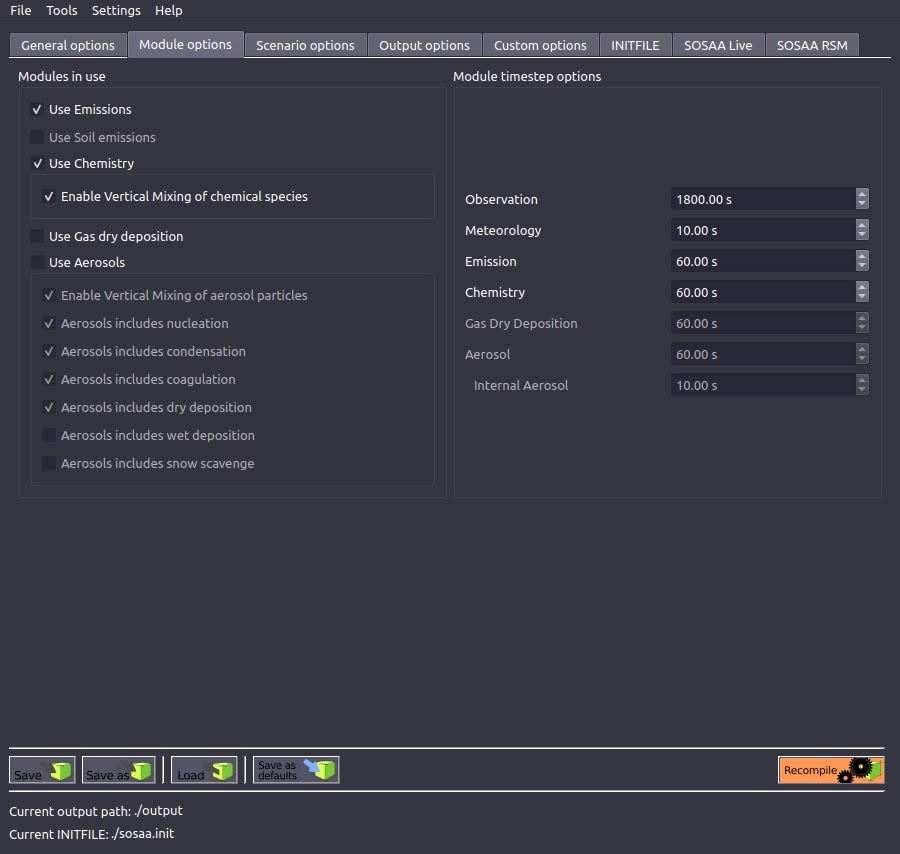
\includegraphics[width=0.475\textwidth]{sosaa-gui/figures/sosaa-modules.png}
    \end{subfigure}
    \begin{subfigure}
        \centering
        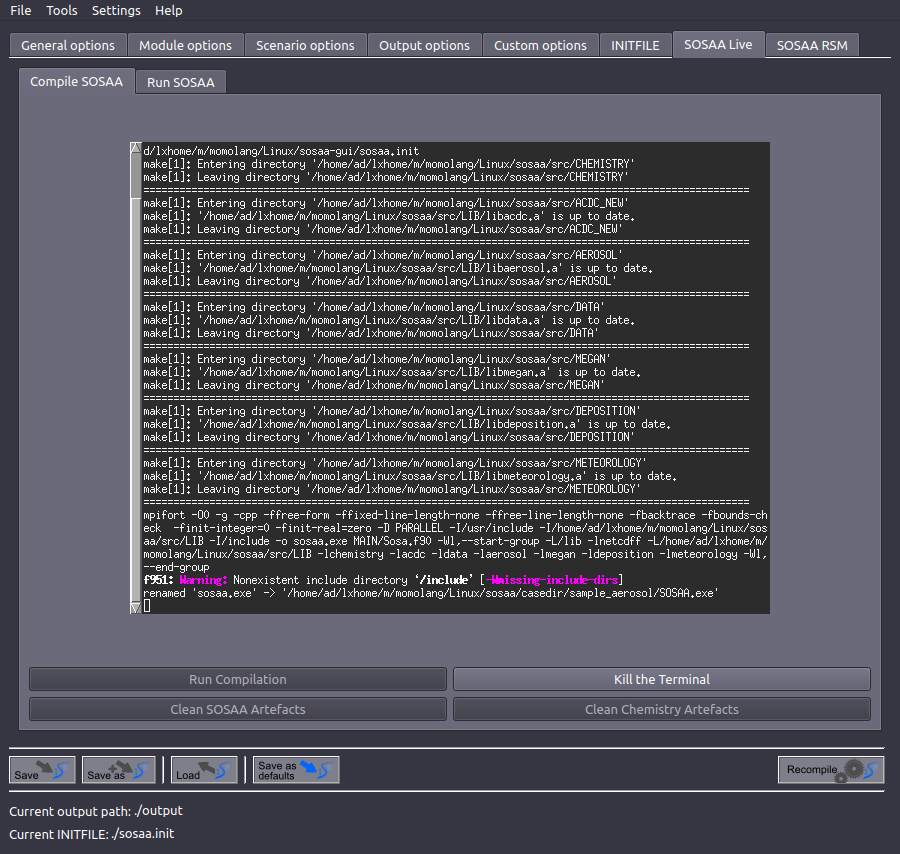
\includegraphics[width=0.475\textwidth]{sosaa-gui/figures/sosaa-compile.png}
    \end{subfigure}

    \caption[Configuring and Compiling SOSAA inside the GUI]{Configuring and Compiling SOSAA inside the GUI. The left screenshot shows the module configuration tab, where the modules used in SOSAA can be enabled, and their timesteps can be set. The right screenshot shows compilation inside an embedded terminal at the press of a button.}
    \label{fig:sosaa-gui-modules-compile}
\end{figure}

\section{Compiling and Running SOSAA from within the GUI} \label{txt:sosaa-gui-compile-run}

The SOSAA GUI is not tightly coupled with the SOSAA model but instead only produces the configuration file that SOSAA reads in. This separation allows the GUI and the model to be independent and run on different systems. However, compiling and running the model from within the GUI can sometimes be more convenient. For instance, the GUI's knowledge of the runtime setup of the model can be used to configure the compilation process as well. Launching large SOSAA runs is still best done from a terminal within an HPC system using the settings file produced a priori using the GUI. On the other hand, launching them from the same system that runs the GUI can be faster and more convenient for quick demo or test runs.

Thus, the GUI comes with two additional tabs for compiling and running SOSAA, which offer a few additional configuration options. The SOSAA GUI utilises the terminal emulators \texttt{xterm} and \texttt{rxvt} to embed terminals session within these tabs. When the user wants to compile or run the model, a new terminal is launched to execute the necessary command, which is constructed by the GUI. Note that even though the GUI here only provides the command and its options, it still transforms the task from having to manually remember and type these options every time into a single click of a button.

\section{Training and Predicting with the SOSAA RSM} \label{txt:sosaa-gui-icarus}

The SOSAA GUI also has optional support for training, evaluating, and using the SOSAA RSM described in \Cref{txt:icarus-evaluation-chapter}. The SOSAA RSM comes with additional dependencies on \texttt{matplotlib} \cite{matplotlib-2007}, \texttt{numpy} \cite{numpy-2020}, \texttt{pandas} \cite{pandas-2010}, \texttt{scipy} \cite{scipy-2020}, and \texttt{sklearn} \cite{scikit-learn-2011, sklearn-api-2013}, which come with significant initial load times. To keep GUI launch times as low as possible and allow users to only use the GUI for configuring SOSAA, these dependencies are kept optional and only loaded lazily when the user interacts with the SOSAA RSM interface. If the optional dependencies have not yet been installed, the user is presented with a helpful error message.

The GUI exposes several options for configuring the training and prediction processes of the RSM, including where the RSM and its predictions are saved, how many trees are included in the random forest predictor, and how many bootstrap samples should be used. Both training and prediction also support seeding their respective random number generators to ensure reproducibility. The GUI provides progress updates during RSM training and prediction to communicate wait times. Once the training has finished, the RSM is evaluated on disjoint training and test sets from the provided dataset. It is worth remembering that the SOSAA RSM implements the Icarus architecture (see \Cref{txt:icarus-rsm}) and thus reports uncertainty levels and confidence scores with every prediction. Using the Monte Carlo analysis approach described in \Cref{txt:icarus-propagation}, the prediction uncertainties and confidence scores are propagated through the RSM evaluation into the analysis results, as can be seen in the lower half of the left screenshot in \Cref{fig:sosaa-gui-rsm-train-results}.

\begin{figure}[H]
    \centering
    \begin{subfigure}
        \centering
        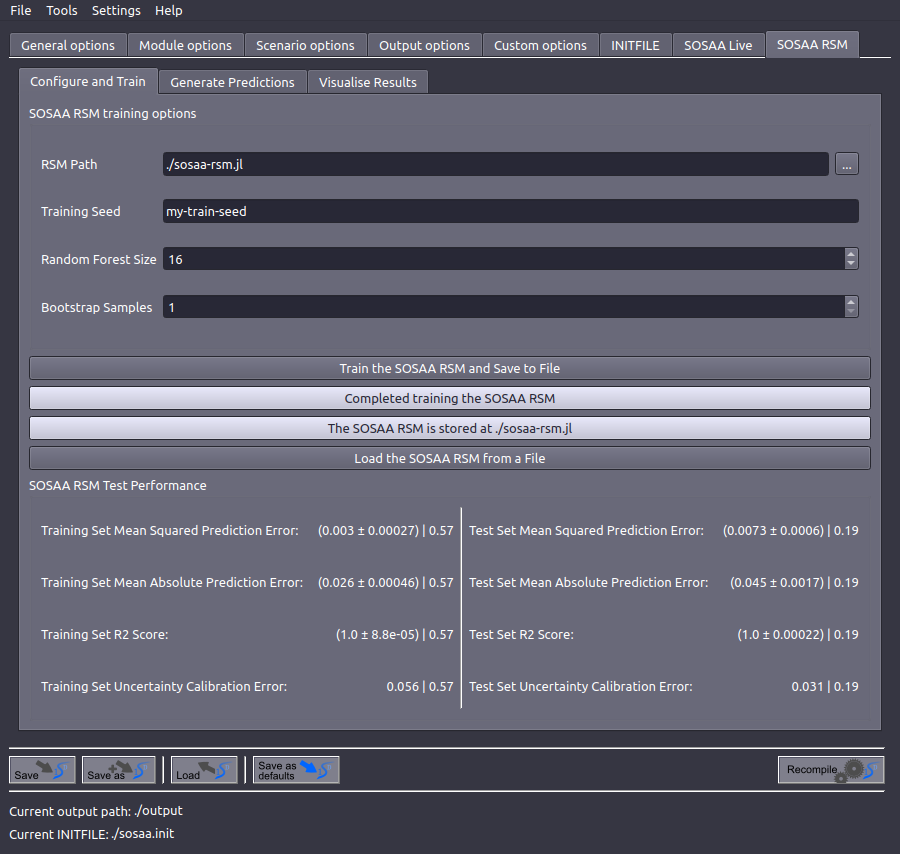
\includegraphics[width=0.475\textwidth]{sosaa-gui/figures/sosaa-rsm-train.png}
    \end{subfigure}
    \begin{subfigure}
        \centering
        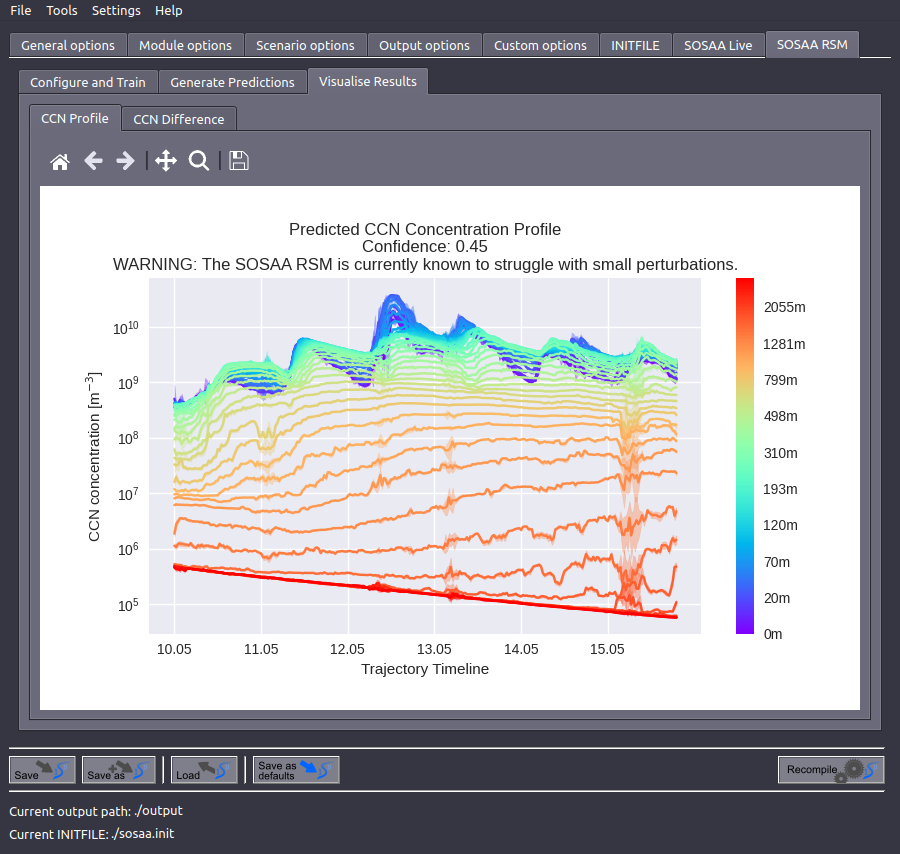
\includegraphics[width=0.475\textwidth]{sosaa-gui/figures/sosaa-rsm-ccn.png}
    \end{subfigure}

    \caption[Training and Predicting with the SOSAA RSM inside the GUI]{Training and Predicting with the SOSAA RSM inside the GUI. The left screenshot shows the SOSAA RSM configuration and training tab, where an RSM can be loaded from a file or trained with data from the SOSAA model and where the RSM's train-test performance is evaluated. After generating a prediction for a user-given change in SOSAA inputs, the CCN profile or change in CCN can be plotted, as shown in the right screenshot.}
    \label{fig:sosaa-gui-rsm-train-results}
\end{figure}

\noindent Once an RSM has been trained, it can be used from within the GUI to predict the CCN concentration on different inputs. In particular, the user specifies a short Python code snippet to calculate the new inputs. The RSM is then invoked on the updated inputs once per requested bootstrap sample, after which uncertainty and confidence propagation is used to combine the predictions. The resulting $(\hat{y} \pm \sigma) \given c$ predictions are plotted inside the GUI for initial inspection, and stored to disk for further downstream analysis. The right screenshot in \Cref{fig:sosaa-gui-rsm-train-results} showcases one such prediction result figure, which plots the predicted CCN profile across the trajectory, mirroring \Cref{fig:six-trajectories-ccn}. Plotting the individual per-prediction change in CCN concentration is also possible and visually communicates point uncertainty and confidence using point clouds and transparency.

\newpar The SOSAA GUI has been designed to make interacting with the SOSAA model more interactive. In particular, users can now explore what-if scenarios using the SOSAA RSM. The GUI also contains the infrastructure to support quickly training and applying future variants of the SOSAA RSM to explore how different inputs may change the SOSAA results. Based on this RSM-aided exploration, the user can then configure and perform new SOSAA runs of particular interest, all without exiting the GUI. We thus hope it to be a valuable tool in future atmospheric and climate science research.
